%  FICHIER  :   template_fira_two_cols.tex
%  A copier à côté des autres .tex et à déclarer dans config.json
% ------------------------------------------------------------------
\documentclass[11pt,a4paper]{article}

% ─── pack de base ─────────────────────────────────────────────────
\usepackage[T1]{fontenc}
\usepackage[utf8]{inputenc}
\usepackage{textcomp}
\usepackage{newtxtext}
\usepackage[british]{babel}
\usepackage[left=0mm,right=0mm,top=0mm,bottom=0mm]{geometry}
\usepackage[stretch=25,shrink=25,tracking=true,letterspace=30]{microtype}
\usepackage{graphicx,xcolor,marvosym,enumitem,paracol,hyperref}
\usepackage{FiraSans}
\renewcommand{\familydefault}{\sfdefault}
\usepackage{array} 
\usepackage{tabularx}
\usepackage{ragged2e}
 \usepackage{fontawesome}
% ─── couleurs & listes ────────────────────────────────────────────
\definecolor{cvblue}{HTML}{304263}
\setlist{parsep=0pt,topsep=0pt,partopsep=1pt,itemsep=1pt,leftmargin=6mm}
\hypersetup{colorlinks=true,urlcolor=white,linkcolor=white}

% ─── macros maison (identiques au modèle original) ────────────────
\newcommand{\dates}[1]{\hfill\textbf{#1}}
\newcommand{\is}{\par\vskip.5ex plus .4ex}
\newcommand{\smaller}[1]{{\small$\diamond$\ #1}}
\newcommand{\headleft}[1]{\vspace*{3ex}\textsc{\textbf{#1}}\par%
  \vspace*{-1.5ex}\hrulefill\par\vspace*{0.7ex}}
\newcommand{\headright}[1]{\vspace*{2.5ex}\textsc{\Large\color{cvblue}#1}\par%
  \vspace*{-2ex}{\color{cvblue}\hrulefill}\par}

% ─── défaut de secours si sidetext absent dans d’autres modèles ───
\providecolor{sidetext}{rgb}{0,0,0}
\definecolor{maincolor}{HTML}{ffffff}
% ─────────────────────────── DOCUMENT ─────────────────────────────
\begin{document}
\thispagestyle{empty}
\setlength{\topskip}{0pt}\setlength{\parindent}{0pt}\setlength{\parskip}{0pt}
\raggedbottom

\begin{minipage}[t]{0.33\textwidth}
  % Bande bleue d’en-tête
  \colorbox{cvblue}{\begin{minipage}[t][5mm][t]{\textwidth}\null\end{minipage}}
  \vspace{-.2ex}
  \colorbox{cvblue!90}{%
    \color{white}\kern0.09\textwidth
    \begin{minipage}[t][293mm][t]{0.82\textwidth}\raggedright
      \vspace*{2.5ex}
      % -------- Identité ------------------------------------------
      \Large Judikael Mourovin\normalsize

      % Photo (s’affiche seulement si 7c85085139e24fcd88b314d882b3ebd2.png ≠ vide)
      \ifx\relax7c85085139e24fcd88b314d882b3ebd2.png\relax\else
        \vspace{2ex}\null\hfill
        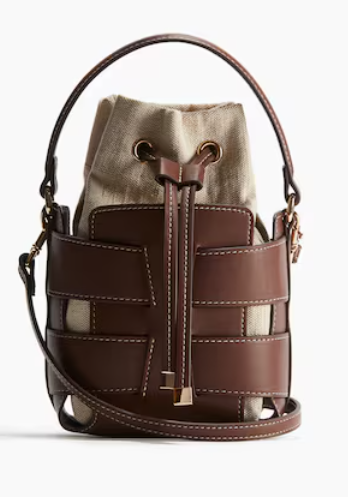
\includegraphics[width=0.65\textwidth]{7c85085139e24fcd88b314d882b3ebd2.png}
        \hfill\null
      \fi

      % -------- Profil -------------------------------------------
      \headleft{Profil}
      \begingroup           % ouvre un groupe local
       \justifying         % rétablit la justification pleine
        Technicien informatique passionné de marketing digital, j’allie administration systèmes, support utilisateurs et conduite de projets numériques. Mon alternance à la DSI de la mairie du Gosier m’a permis d’optimiser les outils internes et d’accompagner la transformation digitale. Autonome, rigoureux et orienté résultat, je souhaite désormais contribuer à la performance numérique et à la satisfaction des utilisateurs au sein d’une organisation dynamique.
      \endgroup             % referme : on revient à \raggedright

      % -------- Contact ------------------------------------------
      \headleft{Contact}\small
      \MVAt\  \texttt{jkmou971@gmail.com}\par
      \Mobilefone\ +590 0690 91 14 48\par
      \Letter\ Route de Cocoyer\par
      97190 Gosier\par
      \faLinkedin\  \href{}{}
      \normalsize

      % -------- Langues (si dispo) -------------------------------
      \ifx\relax\begin{itemize}[leftmargin=*]
\item Anglais - \textcolor{gray}{}
\item Espagnol - \textcolor{gray}{}\end{itemize}\relax\else
        \headleft{Langues}
        \begin{itemize}[leftmargin=*]
\item Anglais - \textcolor{gray}{}
\item Espagnol - \textcolor{gray}{}\end{itemize}
      \fi

      % -------- Compétences --------------------------------------
      \headleft{Compétences}
      \begin{itemize}[leftmargin=*]
\item Administration
\item Maintenance
\item Réseaux
\item Support
\item Marketing
\item Digital
\item Diagnostic\end{itemize}

      % -------- Centres d’intérêt --------------------------------
      \headleft{Intérêts}
      \begin{itemize}[leftmargin=*]
\item Lecture
\item Sport
\item Musique
\item Voyage
\end{itemize}

    \end{minipage}\kern0.09\textwidth
  }
\end{minipage}
% ================================================================
\hskip2.5em
% ======================= COLONNE DROITE =========================
\begin{minipage}[t]{0.56\textwidth}
  \setlength{\parskip}{0.8ex}
  \vspace{2ex}

  % ---------- EXPERIENCE ----------------------------------------
  \headright{Expérience}
  \colorbox{maincolor}{%
  \begin{minipage}{\linewidth}
    \noindent
    \textbf{Alternant en marketing digital}\hfill 09/2023 - 08/2024\\
    Mairie du Gosier – DSI\\[-0.3em]
    \begin{itemize}[leftmargin=*]
      \item Coordination des parties prenantes pour les projets numériques municipaux. \item Analyse des besoins utilisateurs et déploiement de solutions améliorant la productivité. \item Support et formation favorisant l’adoption des outils et de la stratégie digitale.
    \end{itemize}
  \end{minipage}}

\vspace{3mm}

\colorbox{maincolor}{%
  \begin{minipage}{\linewidth}
    \noindent
    \textbf{Animateur de la zone informatique}\hfill 11/2022 - 08/2023\\
    Pôle emploi, Gosier\\[-0.3em]
    \begin{itemize}[leftmargin=*]
      \item Assistance quotidienne et support technique auprès des demandeurs d’emploi. \item Configuration et maintenance des postes pour assurer la disponibilité de l’espace numérique. \item Diagnostic et résolution d’incidents réduisant les temps d’arrêt.
    \end{itemize}
  \end{minipage}}

\vspace{3mm}

\colorbox{maincolor}{%
  \begin{minipage}{\linewidth}
    \noindent
    \textbf{Stagiaire informaticien}\hfill 02/2021 - 05/2021\\
    Numerika, Baie-Mahault\\[-0.3em]
    \begin{itemize}[leftmargin=*]
      \item Installation et entretien des équipements informatiques garantissant leur bon fonctionnement. \item Support de proximité améliorant la réactivité aux demandes internes.
    \end{itemize}
  \end{minipage}}        % ← déjà formaté par build_placeholders()

  % ---------- EDUCATION -----------------------------------------
  \headright{Formation}
  \colorbox{maincolor}{%
  \begin{minipage}{\linewidth}
    \noindent
    \textbf{Bachelor Marketing Digital}\hfill 09/2023 - 08/2024\\
    CFA IUTS\\[-0.3em]
    \begin{itemize}[leftmargin=*]
      \item Stratégies de communication en ligne, gestion de contenu. \item Analyse de données et optimisation de campagnes. \item Gestion de projet web et marketing automation.
    \end{itemize}
  \end{minipage}}

\vspace{3mm}

\colorbox{maincolor}{%
  \begin{minipage}{\linewidth}
    \noindent
    \textbf{BTS Systèmes numériques – option informatique et réseaux}\hfill 09/2019 - 06/2021\\
    Lycée Chevalier Saint-Georges, Les Abymes\\[-0.3em]
    \begin{itemize}[leftmargin=*]
      \item Architecture réseau et administration systèmes. \item Maintenance matériel et logiciel des postes de travail. \item Déploiement de services et sécurisation des infrastructures.
    \end{itemize}
  \end{minipage}}

\end{minipage}

\end{document}
